\documentclass[10pt, landscape, a4paper]{article}
\usepackage{geometry}[landscape]
\usepackage{multicol}
\usepackage{graphicx}
\usepackage{amsmath} 
\usepackage{amssymb}
\usepackage{ccicons}
\usepackage{hyperref}

\usepackage[dvipsnames]{xcolor}

% Set page margins
\geometry{top=.8cm, left=.8cm, right=.8cm, bottom=.8cm}

% Set paragraph indentation
\setlength{\parindent}{0pt}

% Set path for assets
\graphicspath{{assets/}}

\setlength{\columnsep}{20pt}
\raggedcolumns

% _____ CUSTOM COMMANDS __________________________________________
\newcommand{\E}[0]{\mathbb{E}}
\newcommand{\R}[0]{\mathbb{R}}

\newcommand{\sgn}[0]{\text{sgn}}

\newcommand{\argmin}[1]{\underset{#1}{\text{argmin}}}
\newcommand{\argmax}[1]{\underset{#1}{\text{argmax}}}

\begin{document}
\begin{multicols*}{3}

% _____ CONTENT __________________________________________________

% main heading
\begin{center}
	\Large{\textbf{Computer Systems}} \\
    \small{by dcamenisch}
\end{center}

\section{Introduction}

This document is a summary of the 2022 edition of the lecture \textit{Computer Systems} at ETH Zurich. I do not guarantee correctness or completeness, nor is this document endorsed by the lecturers. If you spot any mistakes or find other improvements, feel free to open a pull request at \url{https://github.com/DannyCamenisch/systems-summary}. This work is published as CC BY-NC-SA.

\begin{center}
	\ccbyncsa
\end{center}
\section{Naming}

Naming is a fundamental concept, it allows resources to be bound at different times. Names are bound to objects, this is always relative to a context. One example of this would be path names, e.g. \textit{/usr/bin/emacs}. Name resolution can be seen as a function from context and name to some object. The resolved object can be a context in itself. This gives us a naming network.
\begin{center}
	\includegraphics[width=0.8\linewidth]{naming-network.png}
\end{center}

Both synonyms (two names bound to the same object) and homonyms (the same name bound to two different objects) can occur.
\section{The Kernel}

There are three main functions to an OS. Commonly they are referred to from a designer's view, but the user's view can be much more helpful to actually understand how it works.

\begin{center}
	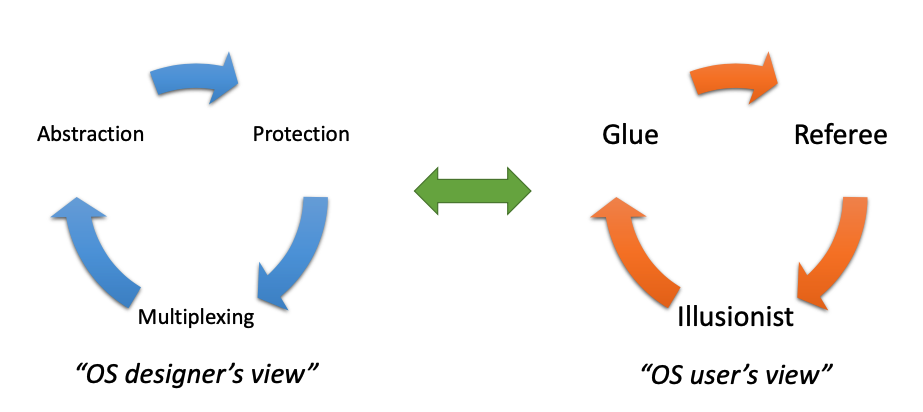
\includegraphics[width=\linewidth]{os-functions.png}
\end{center}


\subsection{Bootstrapping}

The term bootstrapping refers to pulling himself up from his own boots. In computer systems it is what we call the process of starting up a computer (booting). This boot process looks like this:

\begin{enumerate}
	\item CPU starts executing code at a fixed address (Boot ROM)
	\item Boot ROM code loads 2nd stage boot loader into RAM
	\item Boot loader loads kernel and optionally initials file system into RAM
	\item Jumps to kernel entry point
\end{enumerate}

The first few lines are always written in assembly, but generally we want to switch to C as soon as possible.


\subsection{Mode Switch}

One of our main goals is to protect the OS from applications that could harm it (intentionally or not). For this purpose we introduce two different modes:

\begin{itemize}
	\item \textbf{Kernel Mode} - execution with full privileges, read/write to any memory, access and I/O, etc. Code here must be carefully written
	\item \textbf{User Mode} - limited privileges, only those granted by the OS kernel
\end{itemize}

These two (or more) modes are already implemented in hardware. The main reason for a mode switch is when we encounter a processor exception (mode switch from user to kernel mode). If this is the case, we want the following to happen:

\begin{enumerate}
	\item Finish executing current instruction
	\item Switch mode from user to kernel
	\item Look up exception cause in exception vector table
	\item Jump to this address
\end{enumerate}

Further we may also want to save the registers and switch page tables. When switching between the modes we also have to change our address space, but we might want to access some informations from the user mode address space. One way of doing this is to use a so called \textbf{trampoline}, which is a part of the address space that gets mapped to the same location in user and kernel mode.

\begin{center}
	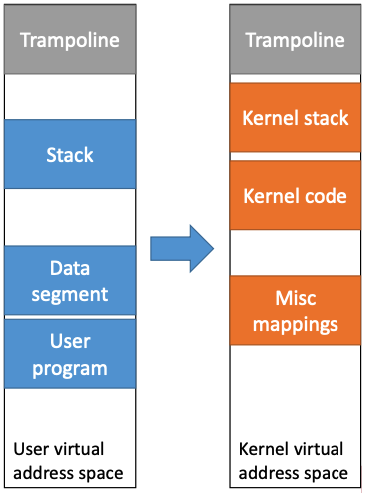
\includegraphics[width=0.4\linewidth]{trampoline.png}
\end{center}

Mode switches can also occur the other way around (from kernel mode to user mode). The main reasons for this are:

\begin{itemize}
	\item New process / thread start
	\item Return from exception
	\item Process / thread context switch
	\item User-level upcall (UNIX signal)
\end{itemize}

This leads us to the following perspective:

\begin{center}
	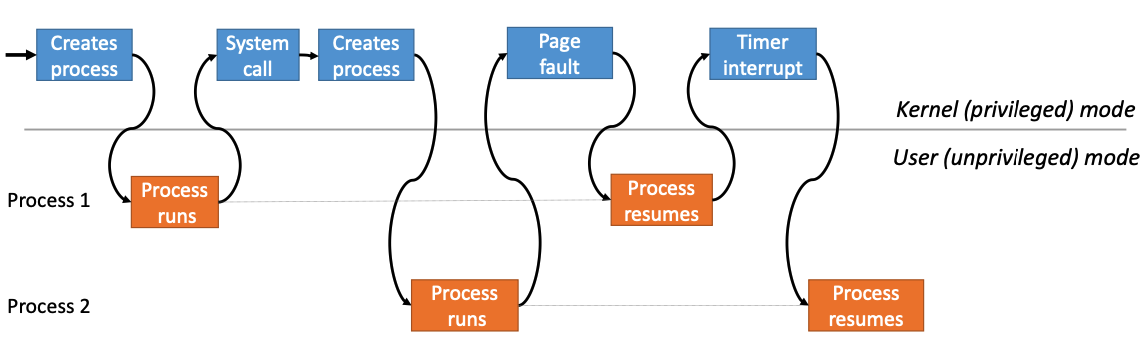
\includegraphics[width=\linewidth]{mode-switch.png}
\end{center}

The mode switch is fundamental to modern computers:

\begin{itemize}
	\item It enables virtualization of the processor
	\item It creates the illusion of multiple computers
	\item It referees access to the CPU
\end{itemize}


\subsection{General Model of OS Structure}

\begin{center}
	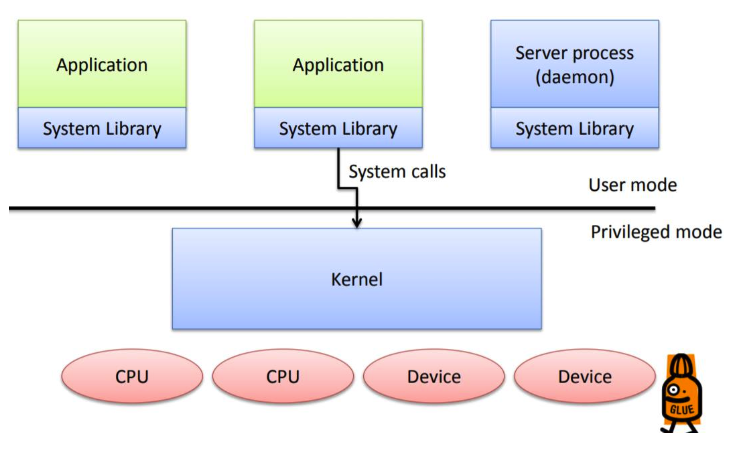
\includegraphics[width=0.9\linewidth]{os-structure.png}
\end{center}

\begin{itemize}
	\item \textbf{Kernel}: The kernel consists of software run in privileged mode. There might be more than one kernel in an OS. It can handle system calls, h/w interrupts etc.
	\item \textbf{System Libraries}: They are part of any application run on the machine and should provide an interface for the kernel.
	\item \textbf{Daemon}: This is a process running as part of the OS. It’s not run in privileged mode and may use system libraries. An example might be a file system.
\end{itemize}

We can differentiate between monolithic kernels and microkernels, depending on the amount of code in kernel mode.


\subsection{System Calls}

System calls are the only way for user mode programs to enter kernel mode. System calls are a type of exception, but they try to look a lot more like a procedure call. Therefore the kernel system call handler has to first locate arguments, copy these arguments into kernel memory, validate these arguments and then copy the results back into user memory after execution. An example of such a system call would be \textit{write()}. 


\subsection{Hardware Timers}

What happens if a user mode program does not cause any exception and does not give control back to the kernel? Hardware timers are a solution for this problem, the hardware device periodically interrupts the processor and returns control to the kernel handler, which sets the time of the next interrupt.

\section{Processes}

When you run a program, the OS creates a process to execute the program in. A process is an illusion created by the OS, it creates an execution environment for a program. This environment gives the program limited rights (access, name spaces, threads, etc.) and therefore it is both a security and a resource principal.


\subsection{Creating a Process}

There are two main approaches to creating new processes:

\begin{itemize}
	\item \textbf{Spawn} - constructs a running process from scratch
	\item \textbf{Fork / Exec} - creates a copy of the calling process or replaces the current program with another in the same process
\end{itemize}

\textbf{Spawn}

\begin{itemize}
	\item Create and initialize the process control block (PCB) in the kernel
	\item Create and initialize a new address space
	\item Load the program into the address space
	\item Copy arguments into memory in the address space
	\item Initialize the hardware context to start execution at "start"
	\item Inform the scheduler that the new process is ready to run
\end{itemize}

Spawn is very complex, we have to specify everything about the new environment. If we omit a key argument a new process might have insufficient rights or resources or it might fail to function due to a security fault. \medskip

\textbf{Fork}

Fork on the other hand is less complex. The child process is almost an exact copy of the parent, with a different PID. We know which process we are in from the return value of the \textit{fork()} call ($0$ for child, $>0$ for parent, $<0$ for error). The complete UNIX process management API also includes:

\begin{itemize}
	\item \textit{exec()} - system call to change the program being run by the current process
	\item \textit{wait()} - system call to wait for a process to finish
	\item \textit{signal()} - system call to send a notification to another process
\end{itemize}

In contrast to \textit{spawn()}, here the child revokes rights and access explicitly before \textit{exec()}, further we can use the full kernel API to customize the execution environment.


\subsection{The Process Control Block}

The PCB is the main kernel data structure used to represent a process. It has to hold or refer to the page table, trap frame, kernel stack, open files, program name, scheduling state, PID, etc.


\subsection{Process Context Switching}

Context switching is the process of switching between different processes running in user mode or kernel mode. It is one of the key elements of the illusion that multiple programs can run in parallel. \columnbreak

There are two main reasons for the kernel to switch processes: either when a process has run for too long and gets interrupted by a hardware timer or when a process blocks. The second case happens when a system call can not complete immediately. The process then often calls \textit{sleep()} and other processes can be executed.
\begin{center}
	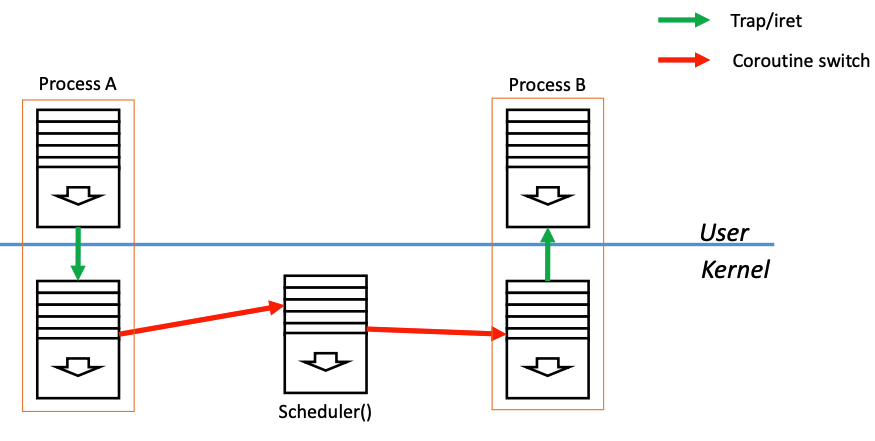
\includegraphics[width=\linewidth]{context-switching.png}
\end{center}


\subsection{Process Hierarchy}

By forking and spawning new processes we create sort of a hierarchy. If a child process dies, but the parent does not call \textit{wait()}, the child process becomes a zombie - it is dead, but still around since nobody asked for the return code. If a parent dies, but the child does not, the child becomes an orphan and gets reparented to the first process (PID \#1, \textit{init}).
\begin{center}
	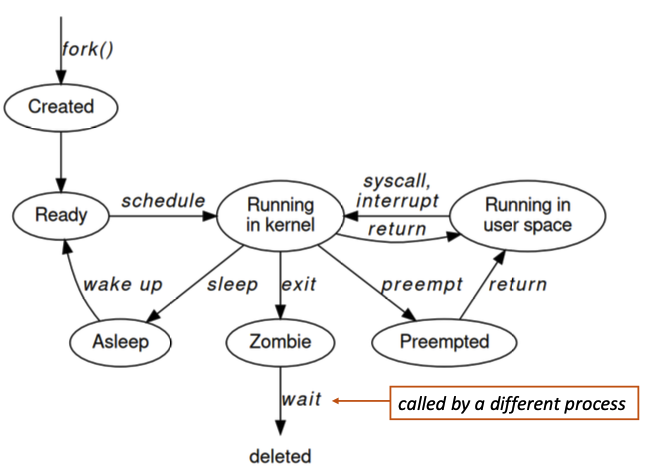
\includegraphics[width=\linewidth]{process-life-cycle.png}
\end{center}

The \textit{init} process is basically an infinite loop calling \textit{wait}(NULL), it gets rid of any zombies.


\subsection{Threads}

Threads are used as an abstraction for concurrency. They allow the usage of parallel hardware, e.g. multiple cores. A thread basically consist of a stack and some register values.\medskip

There is a distinction between \textbf{user threads} and \textbf{kernel threads}. The former are implemented entirely in user’s process. If a user thread is about to block (e.g. when executing a system call), the thread library usually interrupts this call and does something non blocking instead while the system call is served. Kernel threads are implemented by the OS kernel directly. They thus appear as different virtual processors to the user process. In this model, a set of threads share a virtual address space together. Each thread is now scheduled by the kernel itself, which keeps track of threads are part of which process. However, this makes the kernel more complicated.

\section{Inter-Process Communication}

It is often the case, that we want different processes to work together, e.g. DB and web-scraper. For this we need ways to exchange information between processes, we call this inter-process communication or IPC.\medskip

One of the most basic ways to exchange information is system calls. We save our data on the stack or in a register and execute the system call, the kernel then switches execution to the other process with the information about the data that should be exchanged. This is a really flawed approach some reasons are that context switches are expensive and it is unsafe to introduce new system calls for each task.

\subsection{Shared Memory}

We introduce shared memory that can only be accessed by the processes that communicate with each other. This requires us to define a common interface between the processes. The main building blocks for this are:
\begin{itemize}
	\item Shared area: registers, memory - define the layout of the memory
	\item Indicating status: shared variables, signals
	\item Updating status: changing variables
	\item Consistency: use synchronization primitives
\end{itemize}

When checking the state of a shared variable polling can be very inefficient. As an alternative we can use a signal handler. When the first process calls the signal handler, the kernel notifies the second process of the update. When the kernel issues such a system call to a process, we call it an \textbf{upcall}. To guarantee consistency, we use synchronization primitives that are already known from previous lectures (spin locks with CAS, TAS, etc.). \medskip

A more modern approach is to use transactional memory, hereby we work with transactions that can fail on race condition.

\section{Scheduling}

First we introduce some terminology, notice how the wait time is defined as the combination of hold time and execution time.
\begin{center}
	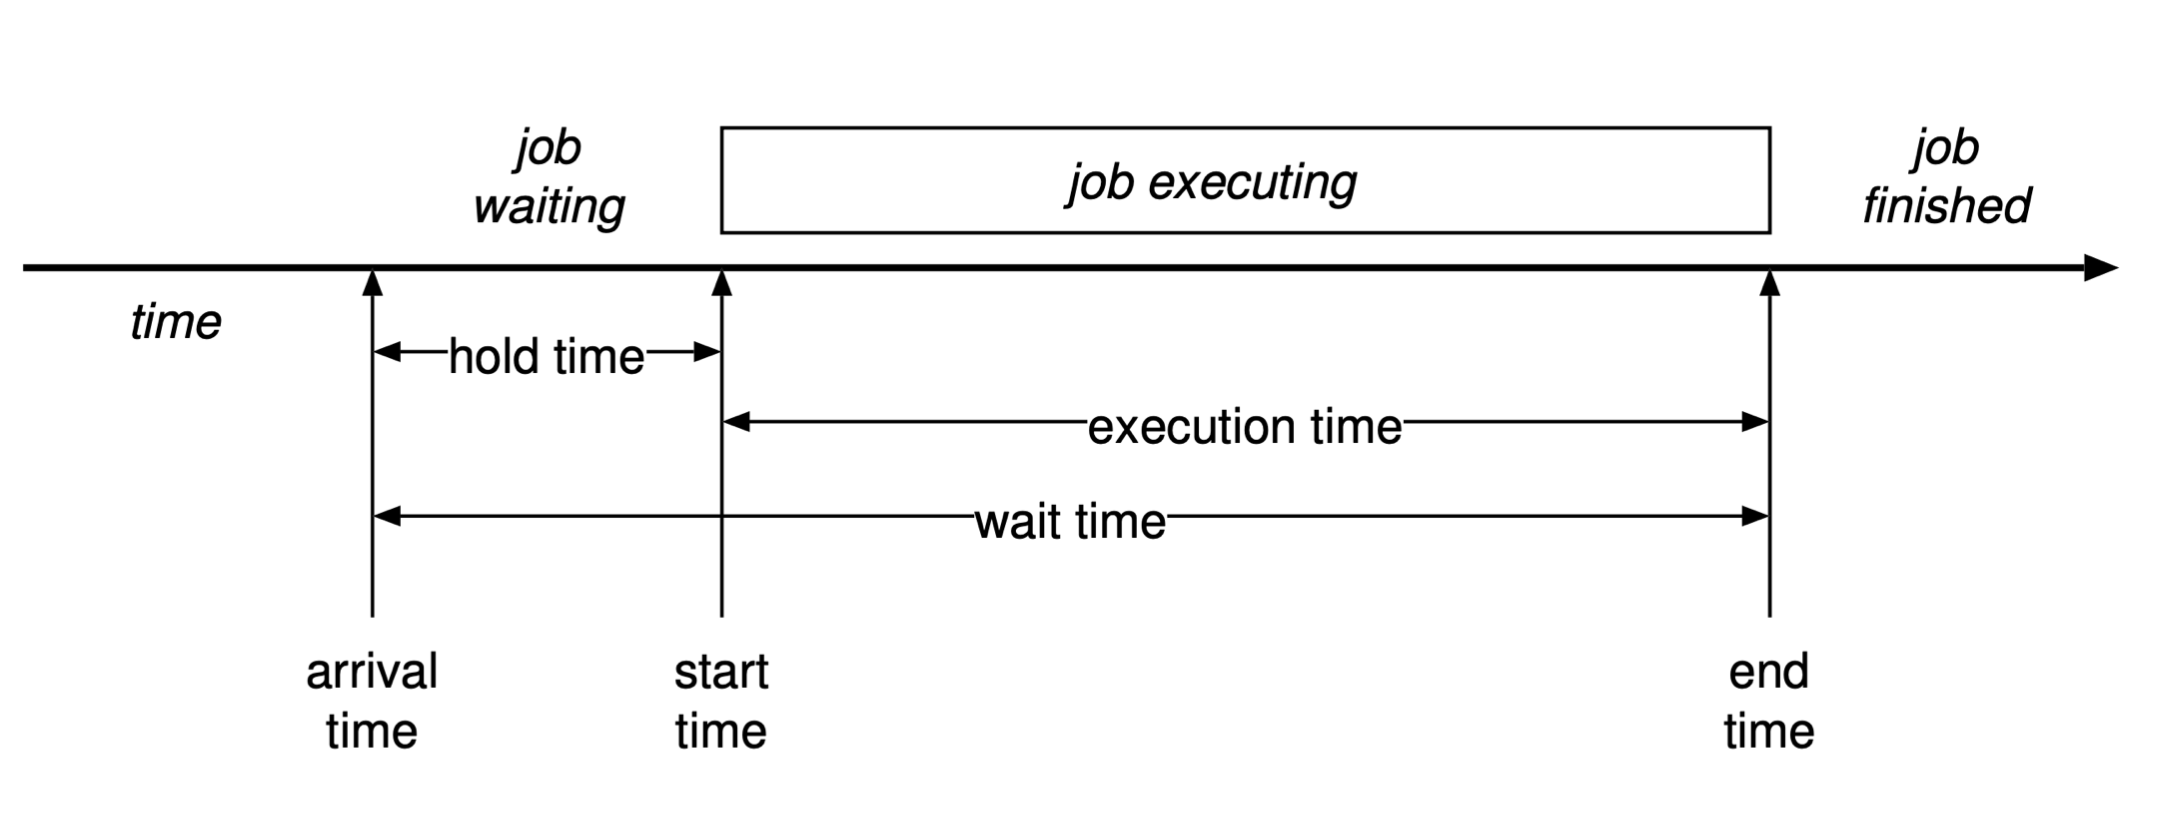
\includegraphics[width=\linewidth]{scheduling.png}
\end{center}

The important metrics for scheduling are throughput (rate of completing jobs) and overhead (time spent without a job executing).

In the following part we will look at various scheduling algorithms, starting from a very simple approach.

\subsection{Non-Preemptive Batch Oriented}

There are two basic algorithms:
\begin{itemize}
	\item First Come First Served
	\item Shortest Job First
\end{itemize}

Both are algorithms are very simple to implement but their applications are limited.

\subsection{Preemptive Batch Oriented}

We introduce preemption, meaning that we interrupt the execution after some finite time interval. After such an interrupt we decide which program to run next. \smallskip

\textbf{Modified SJF:} Go through the sorted list of jobs and execute each until interrupted. Note that the length of a job does not get recomputed after an execution. \smallskip

\subsection{Interactive Scheduling}

When running interactive workload, we can encounter events that block the execution (I/O, page-faults, etc.). During this time we would like to run another program instead of wasting execution time. \smallskip

\textbf{Round Robin Scheduling:} Let $R$ be a queue and $q$ be the scheduling quantum:
\begin{enumerate}
	\item Set an interval timer for an interrupt $q$ seconds in the future
	\item Dispatch the job at the head of $R$
	\item If blocking happens or the timer runs out, return to the scheduler
	\item Push the previously running job to the tail of $R$
\end{enumerate}

\textbf{Priority Based Scheduling:} We assign a priority to each task and dispatch the highest priority task first, if we have ties we use RR to break them. To avoid starvation we might want to use dynamic priorities (increased priority depending on wait time). An even more complex approach is to introduce multi-level queues, meaning that we have a fixed number of queues that assign priorities within each queue. Then we use RR scheduling between the queues to execute tasks. \medskip

Priority scheduling runs into problems when a high priority process has to wait for a lock from a low priority process (Priority Inversion). To fix this, we can either introduce inheritance - the holder of the lock acquires the priority of the highest waiting process - or ceiling - the holder of the lock runs at the highest priority.

\subsection{Linux o(1) Scheduler}

Linux uses 140 multilevel feedback queues, each with a different priority. Multilevel feedback queues penalize CPU bound tasks and prioritize I/O operations, as I/O tasks will eventually block.

The priority range 0-99 is used for high priority, static tasks and it uses FCFS or RR scheduling. The range 100-139 is for user tasks and uses RR together with priority ageing for I/O tasks.


\section{Input / Output}

Every OS has an I/O subsystem, which handles all interaction between the machine and the outside world. The I/O subsystem abstracts individual hardware devices to present a more or less uniform interface, provides a way to name I/O devices, schedules I/O operations and integrates them with the rest of the system, and contains the low-level code to interface with individual hardware devices. \medskip

To an OS programmer, a \textbf{device} is a piece of hardware visible from software. It typically occupies some location on a bus or I/O interconnect, and exposes a set of hardware registers which are either memory mapped or in I/O space. A device is also usually a source of interrupts, and may initiate Direct Memory Access (DMA) transfers. \medskip

The \textbf{device driver} for a particular device is the software in the OS which understands the specific register and descriptor formats, interrupt models, and internal state machines of a given device and abstracts this to the rest of the OS.

\subsection{Data Transfer}

\textbf {Programmed I/O} consists of causing input/output to occur by reading/writing data values to hardware registers. This is the simples form of communication. It is fully synchronous, so the CPU always has to be involved. Further it is polled, the device has no way to signal that new data is ready. \medskip

\textbf{Interrupts} can be used to signal the availability of new data and solve the polling problem. But the problem of CPU involvement still persists.
\begin{center}
	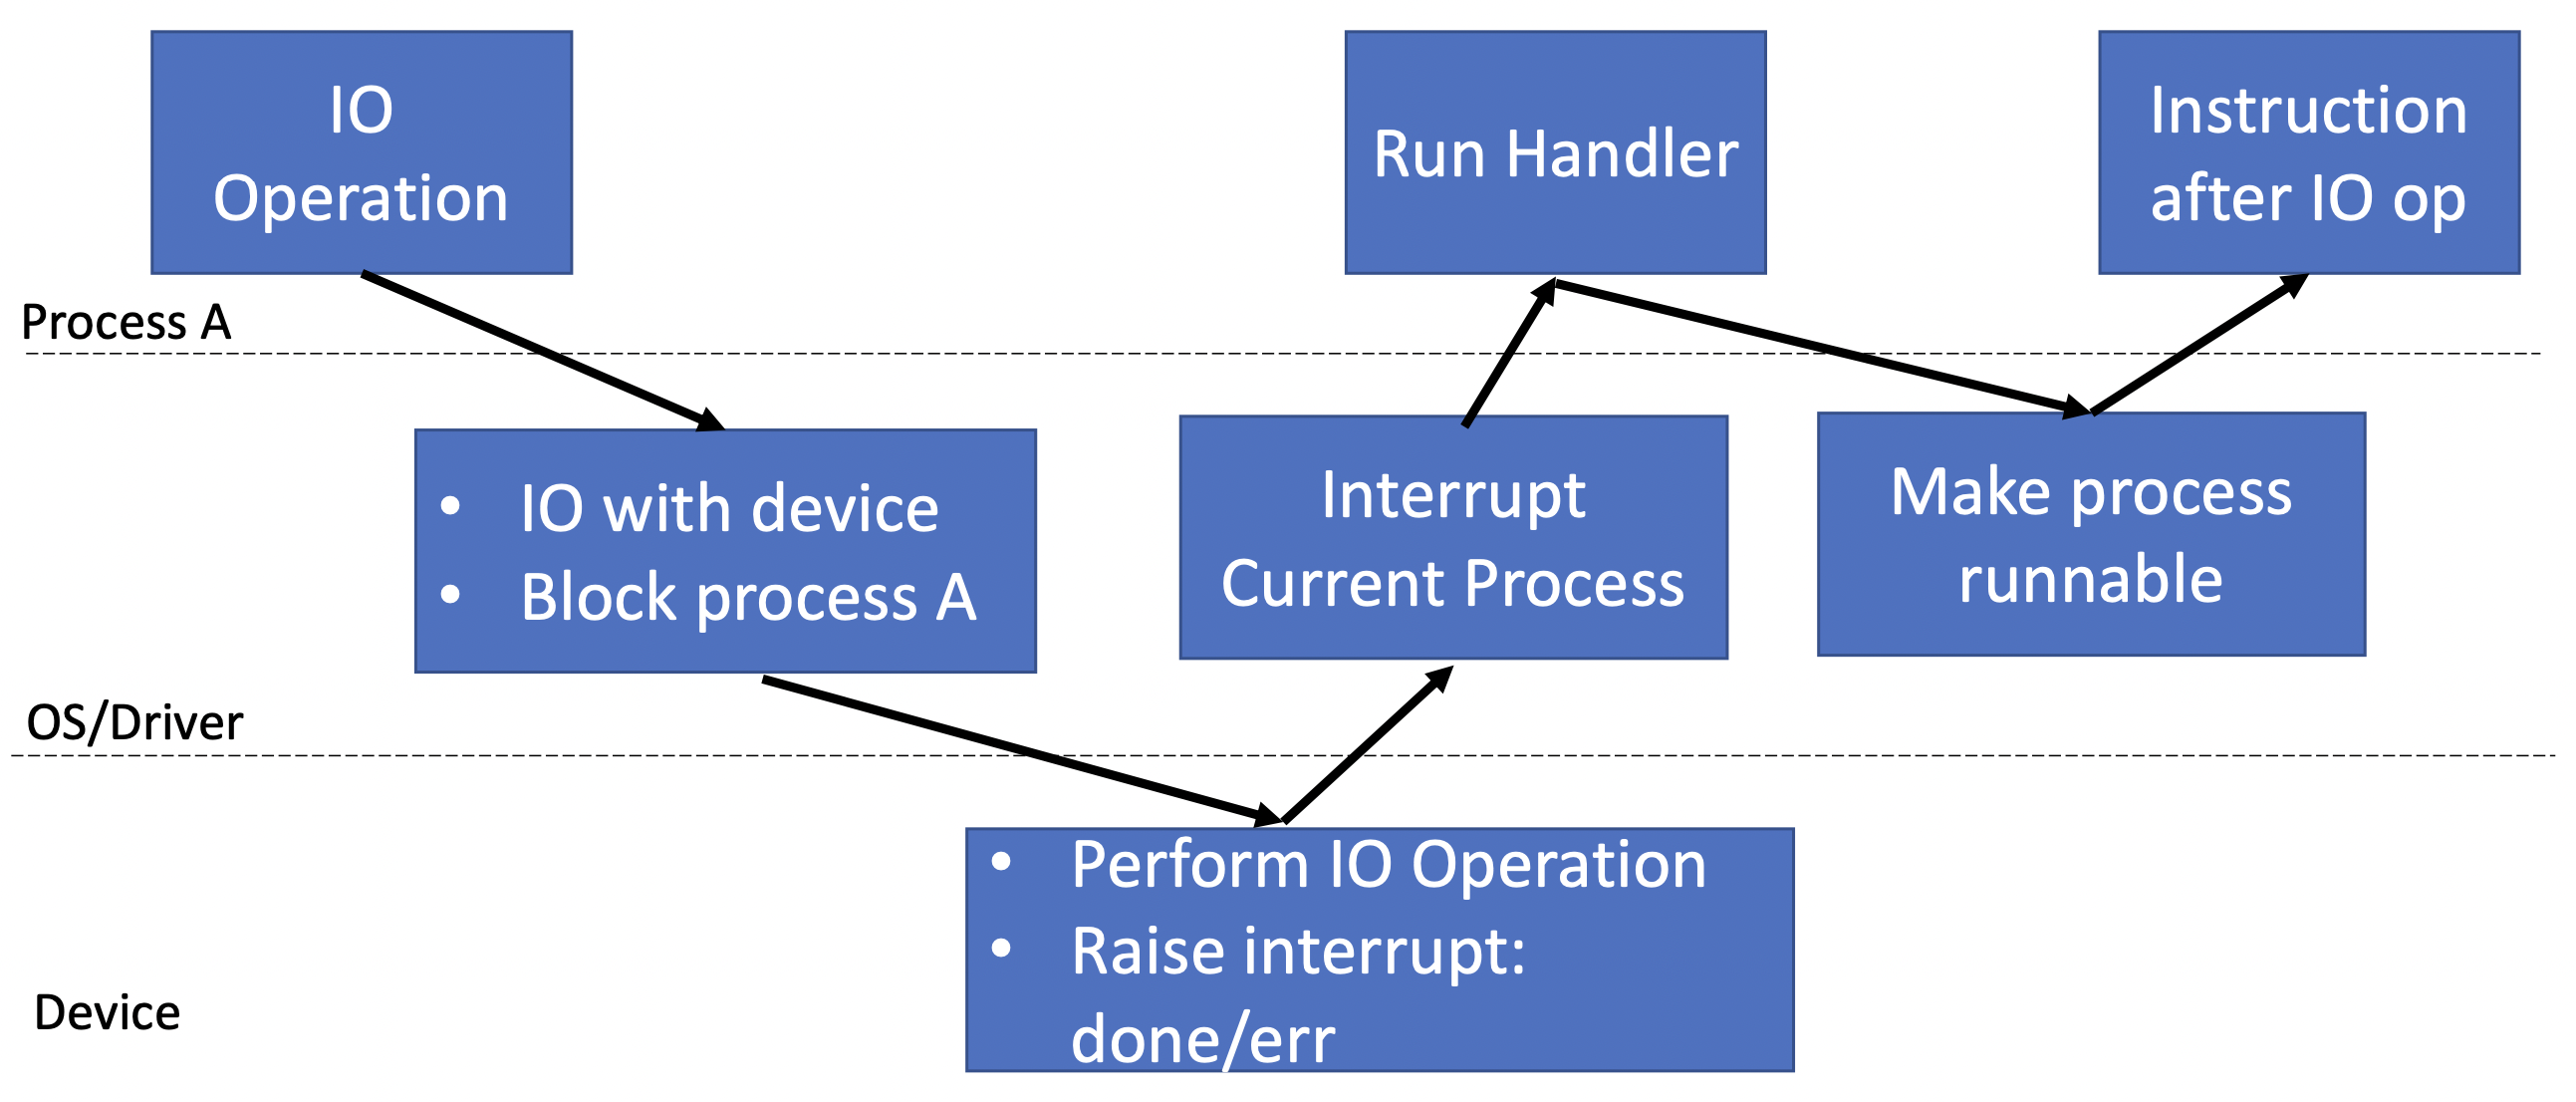
\includegraphics[width=\linewidth]{data_transfer_interrupt.png}
\end{center}

\textbf{Direct Memory Access} or DMA, a device can be given a pointer to buffers in main memory and transfer data to and from those buffers without further involvement from the CPU. A single interrupt is used to signal the end of data transfer. DMA is, for the most part, physical (not virtual) access to memory. Further DMA transfers to and from main memory may or may not be coherent with processor caches.

\subsection{Asynchrony}

Device drivers have to deal with the fundamentally asynchronous nature of I/O: the system must respond to unexpected I/O events, or to events which it knows are going to happen, but not when. \medskip

The \textbf{First-level Interrupt Service Routine} (FLISR) is the code that executes immediately as a result of the interrupt. It runs regardless of what else is happening in the kernel. As a result, it can't change much since the normal kernel invariants might not hold. \medskip

Since I/O is for the most part interrupt-driven, but data is transferred to and from processes which perform explicit operations to send and receive it. Consequently, data must be buffered between the process and the interrupt handler, and the two must somehow rendezvous to exchange data. There are three canonical solutions to this problem:

A \textbf{deferred procedure call}, is a program closure created by the 1st-level interrupt handler. It is run later by any convenient process, typically just before the kernel is exited. \medskip

A \textbf{driver thread}, sometimes called an interrupt handler thread, serves as an intermediary between ISR and processes. The thread starts blocked waiting for a signal either from the user process or the ISR. When an interrupt occurs or a user process issues a request, the thread is unblocked (this operation can be done inside an ISR) and it performs whatever I/O processing is necessary before going back to sleep. Driver threads are heavyweight: even if they only run in the kernel, the still require a stack and a context switch to and from them to perform any I/O requests. \medskip

The third alternative, is to have the FLISR convert the interrupt into a message to be sent to the driver process. This is conceptually similar to a DPC, but is even simpler: it simply directs the process to look at the device. However, it does require the FLISR to synthesize an IPC message, which might be expensive. In non-preemptive kernels which only process exceptions serially, however, this is not a problem, since the kernel does not need locks. \medskip

\textbf{Bottom-half handler} - the part of a device driver code which executes either in the interrupt context or as a result of the interrupt. \medskip

\textbf{Top-half handler} - the part of a device driver which is called "from above", i.e. from user or OS processes.

\subsection{Device Models}

The device model of an OS is the set of key abstractions that define how devices are represented to the rest of the system by their individual drivers. It includes the basic API to a device driver, but goes beyond this: it encompasses how devices are named throughout the system, and how their interconnections are represented as well. \medskip

\textbf{UNIX device model:}
\begin{itemize}
	\item Character Devices - used for unstructured I/O and present a byte-stream interface with no block boundaries.
	\item Block Devices - used for structured I/O and deal with blocks of data at a time.
	\item Network Devices - correspond to a network interface adapter. It is accessed through a rather different API.
	\item Pseudo Devices - a software service provided by the OS kernel which it is convenient to abstract as a device, even though it does not correspond a physical piece of hardware.
\end{itemize}

\subsection{Protection}

Another function of the I/O subsystem is to perform protection. Ensuring that only authorized processes can access devices or services offered by the device driver and that a device can't be configured to do something harmful. Unix controls access to the drivers themselves by representing them as files, and thereby leveraging the protection model of the file system. DMA-capable devices are in principle capable of writing to physical memory anywhere in the system, and so it is important to check any addresses passed to them by the device driver. Even if you trust the driver, it has to make sure that it’s not going to ask the device to DMA somewhere it shouldn’t. One approach is to put a memory management unit (MMU) on the path between the device and main memory, in addition to each core having one.


\end{multicols*}
\end{document}

% ____ FOOTER ______________________________________________________
% Content and Template: 
% original by Danny Camenisch (dcamenisch@inf.ethz.ch), 2022
% based on different summaries from many helpful people